\documentclass[11pt, a4paper]{article}
\usepackage[utf8]{inputenc}
\usepackage{amsmath,setspace,geometry}
\usepackage{amsthm}
\usepackage{amsfonts}
\usepackage[shortlabels]{enumitem}
\usepackage{rotating}
\usepackage{pdflscape}
\usepackage{graphicx}
\usepackage{bbm}
\usepackage[dvipsnames]{xcolor}
\usepackage{hyperref}
\hypersetup{colorlinks=true, linkcolor= BrickRed, citecolor = BrickRed, filecolor = BrickRed, urlcolor = BrickRed, hypertexnames = true}
\usepackage[]{natbib} 
\bibpunct[:]{(}{)}{,}{a}{}{,}
\geometry{left = 1.0in,right = 1.0in,top = 1.0in,bottom = 1.0in}
\usepackage[english]{babel}
\usepackage{float}
\usepackage{caption}
\usepackage{subcaption}
\usepackage{tikz}
\usepackage{booktabs}
\usepackage{pdfpages}
\usepackage{threeparttable}
\usepackage{lscape}
\usepackage{bm}
\setstretch{1.4}
%\usepackage[tablesfirst,nolists]{endfloat}

\newtheorem{theorem}{Theorem}
\newtheorem{assumption}{Assumption}
\newtheorem{lemma}{Lemma}
\newtheorem{definition}{Definition}
\newtheorem{proposition}{Proposition}
\newtheorem{claim}{Claim}
\newtheorem{corollary}{Corollary}
\newtheorem{example}{Example}
\DeclareMathOperator{\rank}{rank}


\title{Conduct Parameter Estimation in Homogeneous Goods Markets with Equilibrium Existence and Uniqueness Conditions: The Case of Log-linear Specification}
\author{Yuri Matsumura\thanks{Department of Economics, Rice University. Email: Yuri.Matsumura@rice.edu} \and Suguru Otani \thanks{Department of Economics, Rice University. Email: so19@rice.edu
\\Declarations of interest: none %this is for Economics Letters
}}

\begin{document}



\maketitle
\begin{abstract}
    We propose a constrained generalized method of moments estimator (GMM) incorporating theoretical conditions for the unique existence of equilibrium prices for estimating conduct parameters in a log-linear model with homogeneous goods markets. 
    First, we derive such conditions.
    Second, Monte Carlo simulations confirm that in a log-linear model, incorporating the conditions resolves the problems of implausibly low or negative values of conduct parameters.
\end{abstract}

\noindent\textbf{Keywords:} Conduct parameters, Homogenous Goods Market, Mathematical Programming with Equilibrium Constraints, Monte Carlo simulation
\vspace{0in}
\newline
\noindent\textbf{JEL Codes:} C5, C13, L1

\bigskip

\section{Introduction}
Measuring competitiveness is a crucial task in the empirical industrial organization literature.
Conduct parameter is considered a useful measure of competitiveness. 
However, it cannot be directly measured from data because data usually lack information about marginal cost.
Therefore, researchers aim to identify and estimate the conduct parameter.

As the simplest specification, \citet{bresnahan1982oligopoly} considers identification of conduct parameters for the linear model. \cite{matsumura2023resolving} resolves the conflict on some identification problems between \cite{bresnahan1982oligopoly} and \cite{perloff2012collinearity}. 
However, researchers often implement alternative specifications, such as the log-linear model \citep{okazaki2022excess,merel2009measuring}. 
In the context of the log-linear model, these papers identify estimation issues, with some estimated conduct parameters being unrealistically low or even negative.
This raises doubts about the methodology, despite the identification strategy outlined by \citet{lau1982identifying}.
This is an obstacle to choosing a better specification of the demand and supply functions.

To overcome the problem, we propose a constrained generalized method of moments estimator (GMM) incorporating theoretical conditions for the unique existence of equilibrium prices as constraints. 
First, we prove that a unique equilibrium exists under certain theoretical conditions. 
As far as we know, this is a new result.
Second, we show that incorporating equilibrium existence and uniqueness conditions resolves the above estimation problems and makes the model work in estimating conduct parameters even in the log-linear model. 
Hence, our results support those of \cite{lau1982identifying} numerically.


\section{Model}
Consider data with $T$ markets with homogeneous products.
Assume there are $N$ firms in each market.
Let $t = 1,\ldots, T$ be the index of markets.
Then, we obtain the supply equation:
\begin{align}
     P_t = -\theta\frac{\partial P_t(Q_{t})}{\partial Q_{t}}Q_{t} + MC_t(Q_{t}),\label{eq:supply_equation}
\end{align}
where $Q_{t}$ is the aggregate quantity, $P_t(Q_{t})$ is the demand function, $MC_{t}(Q_{t})$ is the marginal cost function, and $\theta\in[0,1]$, which is the conduct parameter. 
The equation nests perfect competition $(\theta=0)$, Cournot competition $(\theta=1 / N)$, and perfect collusion $(\theta=$ $1)$ \citep{bresnahan1982oligopoly}.

Consider an econometric model.
Assume that the demand and the marginal cost functions are written as follows: 
\begin{align*}
    P_t = f(Q_{t}, X^{d}_{t}, \varepsilon^{d}_{t}, \alpha), %\label{eq:demand}
    \\
    MC_t = g(Q_{t}, X^{c}_{t}, \varepsilon^{c}_{t}, \gamma),%\label{eq:marginal_cost}
\end{align*}
where $X^{d}_{t}$ and $X^{c}_{t}$ are the vector of exogenous variables, $\varepsilon^{d}_{t}$ and $\varepsilon^{c}_{t}$ are the error terms, and $\alpha$ and $\gamma$ are the vector of parameters.
We also have the demand- and supply-side instruments, $Z^{d}_{t}$ and $Z^{c}_{t}$, and assume that the error terms satisfy the mean independence condition $E[\varepsilon^{d}_{t}\mid X^{d}_{t}, Z^{d}_{t}] = E[\varepsilon^{c}_{t} \mid X^{c}_{t}, Z^{c}_{t}] =0$. 

\subsection{Log-linear demand and log-linear marginal cost}
Consider a log-linear model, which is a typical specification.
The demand and marginal cost functions are specified as
\begin{align}
    \log P_{t} &= \alpha_0 - (\alpha_1 + \alpha_2 Z^{R}_{t}) \log Q_t + \alpha_3 \log Y_t + \varepsilon^{d}_{t},\label{eq:log_linear_demand}\\
    \log MC_t &= \gamma_0 + \gamma_1 \log Q_t +  \gamma_2 \log W_{t} + \gamma_3 \log R_t + \varepsilon^{c}_{t},\label{eq:log_linear_marginal_cost}
\end{align}
where $Y_{t}$ is an excluded demand shifter, $W_t$ and $R_t$ are excluded cost shifters, and $Z_t^R$ is Bresnahan's demand rotation instrument.
%Since $\partial P_t/\partial Q_t = - (\alpha_1 + \alpha_2 Z_{t}^R) (P_t/Q_t) $, 
Then, Equation \eqref{eq:supply_equation} is written as
\begin{align}
    P_t &= \theta (\alpha_1 + \alpha_2 Z^{R}_{t}) P_t + MC_t.\label{eq:log_linear_supply_equation_direct}
\end{align}

By taking logarithm of Equation \eqref{eq:log_linear_supply_equation_direct} and substituting Equation \eqref{eq:log_linear_marginal_cost}, we obtain
\begin{align}
    \log P_t = - \log(1 - \theta(\alpha_1 + \alpha_2 Z^{R}_{t})) + \gamma_0 + \gamma_1 \log Q_t +  \gamma_2 \log W_{t} + \gamma_3 \log R_t + \varepsilon^{c}_{t}. \label{eq:log_linear_supply_equation}
\end{align}

%An obstacle to estimate parameters is log-transformation in Equation \eqref{eq:log_linear_supply_equation}. First, the standard numerical algorithm faces invalid errors when evaluating the term, $\log (1 - \theta (\alpha_1 + \alpha_2 Z^{R}_{t}))$, whose inner candidate value, $(1 - \theta (\alpha_1 + \alpha_2 Z^{R}_{t}))$, is negative. The problem is inevitable because the true values of parameters are unknown. As in practical situations, researchers may want to use multiple rotation demand instruments or conduct parameters varied with time- or market- fixed effects.\footnote{See \cite{michel2018estimating} for the case of differentiated goods markets.} Then, the problem regarding the term becomes severer because the number of parameters within the log term increases. Second, if researchers may want to specify the demand function as $P_t=\alpha_0-\left(\alpha_1+\alpha_2 Z_t^R\right) Q_t+\alpha_3 Y_t+\varepsilon_t^d$, then the supply equation \eqref{eq:log_linear_supply_equation} is changed to $P_t=\theta \alpha_2 Z_t^R Q_t+\theta \alpha_1Q_t+\exp(\gamma_0+\gamma_1 \log Q_t+\gamma_2 \log W_t+\gamma_3 \log R_t+\varepsilon_t^c)$ which is nonlinear in cost parameters and conduct parameter $\theta$. 
%When constructing moment conditions, researchers face the above problem on log-transformation which limit researchers' alternative set of potential specifications.

% An obstacle in the estimation is log-transformation in Equation \eqref{eq:log_linear_supply_equation}.
% The standard numerical algorithm stops with invalid errors when the inside of the log function, $1 - \theta (\alpha_1 + \alpha_2 Z^{R}_{t})$, becomes negative during the search for an optimizer.
% This problem is not specific to the above model and happens in other specifications, such as a model with linear demand and log-linear marginal cost.

In this model, the number of equilibrium prices varies. 
Although it is a widely known model, to our knowledge, there is no paper examining this.
Thus, we derive the conditions for the uniqueness in the following proposition which are used in our estimation. 
\begin{proposition}\label{prop:equilibrium_existence}
    Assume that $\alpha_1 + \alpha_2 Z^{R}_{t}\ne 0$. Let $\Xi = \gamma_0 + \gamma_1\frac{\alpha_0 + \alpha_3 \log Y_t + \varepsilon^{d}_{t}}{\alpha_1 + \alpha_2 Z^{R}_{t}} +  \gamma_2 \log W_{t} + \gamma_3 \log R_t + \varepsilon^{c}_{t}$.
    The number of equilibrium prices $P_{t}^*>0$ is determined as follows:
    \begin{itemize}
        \item When $1 - \theta (\alpha_1 + \alpha_2 Z^{R}_{t}) \le 0$, there is no equilibrium price,
        \item When $1 - \theta (\alpha_1 + \alpha_2 Z^{R}_{t}) >0$, 
        \begin{itemize}
            \item If $-\gamma_1/(\alpha_1+\alpha_2 Z^R) \ne 1$, there is a unique equilibrium price,
            \item If $-\gamma_1/(\alpha_1+\alpha_2 Z^R) =1$, there are infinitely many equilibrium prices when $\exp(\Xi) = 1 - \theta (\alpha_1 + \alpha_2 Z^{R}_{t})$, but there is no equilibrium price otherwise.
        \end{itemize}
    \end{itemize}
\end{proposition}
See the online appendix \ref{sec:appendix_proof} for the proof.




% \subsection{Log-linear demand and log-quadratic marginal cost}
% Next, we consider more nonlinear specification.
% Assume that the cost function is a log-quadratic form specified as:
% \begin{align}
%     \log MC_t &= \gamma_0 + \gamma_1 \log Q_t + \tilde{\gamma}_1 (\log Q_t)^{2} +  \gamma_2 \log W_{t} + \gamma_3 \log R_t + \varepsilon^{c}_{t}.
% \end{align}
% Then, the log aggregate quantity $\log Q_t $ is a solution of: 
% \begin{align}
%     (\log Q_t)^{2} + \frac{\gamma_1}{\tilde{\gamma}_{1}}\log Q_{t} +\frac{C}{\tilde{\gamma}_{1}} &= 0,
% \end{align}
% where $C=\alpha_0 + \alpha_3 \log Y_t + \log (1 - \theta (\alpha_1 + \alpha_2 Z^{R}_{t})) - \gamma_0  -  \gamma_2 \log W_{t} - \gamma_3 \log R_t + \varepsilon^{d}_{t} - \varepsilon^{c}_{t}$.
% Note that although this specification does not have an analytical solution, we can find numerically find a single positive solution.
\section{Estimation}
To estimate parameters in the demand and supply equations, we use GMM estimation.
Among GMM estimators, we apply the nonlinear system two-stage-least-squares (N2SLS) using Equation \eqref{eq:log_linear_demand} and \eqref{eq:log_linear_supply_equation}.

Let $\xi = (\alpha_0,\alpha_1, \alpha_2, \alpha_3, \gamma_0,\gamma_1, \gamma_2, \gamma_3, \theta)$ be the vector of parameters. 
Given the demand equation \eqref{eq:log_linear_demand} and the supply equation \eqref{eq:log_linear_supply_equation}, we can write the error terms in the demand and supply equation as
\begin{align}
    {\varepsilon}_t^d(\xi) & =  \log P_{t} - \alpha_0 + (\alpha_1 + \alpha_2 Z^{R}_{t}) \log Q_t - \alpha_3 \log Y_t \label{eq:residual_demand_2sls}, \\
    {\varepsilon}_t^c(\xi) & =  \log P_t + \log(1 - \theta(\alpha_1 + \alpha_2 Z^{R}_{t})) -\gamma_0 - \gamma_1 \log Q_t -  \gamma_2 \log W_{t} -\gamma_3 \log R_t \label{eq:residual_supply_2sls}.
\end{align}
To estimate the parameters, we convert the conditional moment conditions, $E[\varepsilon_t^d\mid Z_t^d] = E[\varepsilon_t^c\mid Z_t^c]=0$, into unconditional moment conditions, $E[\varepsilon_t^d Z_t^d] = E[\varepsilon_t^cZ_t^c]=0$.
Using Equations \eqref{eq:residual_demand_2sls} and \eqref{eq:residual_supply_2sls}, we construct the sample analog of the moment conditions:
\begin{align*}
    g(\xi) = \left[\begin{array}{l}
    \frac{1}{T}\sum_{t=1}^T{\varepsilon}^{d}_{t}(\xi)Z_{t}^{d} \\
    \frac{1}{T}\sum_{t=1}^T{\varepsilon}^{c}_{t}(\xi)Z_{t}^{c}
    \end{array}\right].
\end{align*}
We define the GMM estimator as the vector $\xi^*$ that solves the problem,
\begin{align}
    \min_{\xi}\ g(\xi)^\top W g(\xi) \label{eq:minimization_gmm}
\end{align}
where the weight matrix $W$ is defined as
\begin{align}
    W = \left[\frac{1}{T}\sum_{t = 1}^T Z_t^\top Z_t\right]^{-1} \text{ where } Z_{t}=\left[\begin{array}{ll}
        Z_{t}^{d\top} & 0 \\
        0 & Z_{t}^{c\top}
    \end{array}\right].\label{eq:weight_matrix}
\end{align}
The solution to \eqref{eq:minimization_gmm} is called the N2SLS estimator \citep{wooldridge2010econometric}. 

Using Proposition \ref{prop:equilibrium_existence}, we impose the following constraints:
\begin{align}
    &0\le\theta \le 1,\label{eq:conduct_constraint}\\
    &\alpha_1 + \alpha_2 Z_{t}^{R} >0, \quad \gamma_1>0 ,\quad t = 1,\ldots, T\label{eq:slope_constraint}\\
    &1- \theta(\alpha_1 + \alpha_2 Z_{t}^{R}) >0,\quad t = 1,\ldots, T.\label{eq:equlibrium_existence}
\end{align}
Constraint \eqref{eq:conduct_constraint} is a standard assumption on the conduct parameter.
Constraints \eqref{eq:slope_constraint} and \eqref{eq:equlibrium_existence} relate to the uniqueness of equilibrium prices. 
Constraint \eqref{eq:slope_constraint} implies the downward-sloping demand and upward-sloping marginal cost. See online appendix \ref{sec:setting} for the detailed setting.

\section{Simulation results}\label{sec:results}

We compare N2SLS estimation with and without Constraints \eqref{eq:conduct_constraint}, \eqref{eq:slope_constraint}, and \eqref{eq:equlibrium_existence}.
Table \ref{tb:loglinear_loglinear_sigma_1_simultaneous_non_constraint_theta_constraint_bias_rmse} presents the results.
First, as reported in the literature \citep{merel2009measuring,okazaki2022excess}, N2SLS without constraints converges to implausibly low and negative conduct parameters.
This is because the algorithm searches the area in which no equilibrium price and quantity exist and then finds unreasonable local optima that might have a lower objective function than at the true values.
Second, N2SLS with constraints converges to the reasonable values. 
As the sample size increases, the bias and root-mean-square error (RMSE) decrease to levels comparable to linear models.
Third, we find an ad hoc method that uses Equation \eqref{eq:log_linear_marginal_cost} to compute the residual in the supply estimation, $\varepsilon_{t}^c$, and Equation \eqref{eq:log_linear_supply_equation_direct} as an equality constraint with  Constraints \eqref{eq:conduct_constraint}, \eqref{eq:slope_constraint}, and \eqref{eq:equlibrium_existence}. 
Then, the bias and RMSE of conduct parameter $\theta$ are reduced to 0.014 and 0.217 in Panel (c), although the results do not dominate the results in Panel (b) for all parameters.
Therefore, incorporating equilibrium existence and uniqueness conditions simply is helpful for conduct parameter estimation in nonlinear models such as a log-linear model.
See online appendix \ref{sec:additional_experiments} for additional experiments under different variances of errors and the results of a linear model. 

\begin{table}[!htbp]
  \begin{center}
      \caption{Performance comparison}
      \label{tb:loglinear_loglinear_sigma_1_simultaneous_non_constraint_theta_constraint_bias_rmse} 
      \subfloat[N2SLS without Constraints \eqref{eq:conduct_constraint}, \eqref{eq:slope_constraint}, and \eqref{eq:equlibrium_existence}]{
\begin{tabular}[t]{llrrrrrrr}
\toprule
  & Bias & RMSE & Bias & RMSE & Bias & RMSE & Bias & RMSE\\
\midrule
$\alpha_{0}$ & -1.484 & 3.189 & -0.673 & 2.226 & NA & NA & NA & NA\\
$\alpha_{1}$ & -0.850 & 1.781 & -0.452 & 1.199 & NA & NA & NA & NA\\
$\alpha_{2}$ & -0.033 & 0.316 & 0.013 & 0.232 & NA & NA & NA & NA\\
$\alpha_{3}$ & -0.376 & 0.890 & -0.341 & 0.605 & NA & NA & NA & NA\\
$\gamma_{0}$ & 1.295 & 6.875 & 5.380 & 16.505 & NA & NA & NA & NA\\
$\gamma_{1}$ & 0.339 & 1.986 & -0.994 & 6.214 & NA & NA & NA & NA\\
$\gamma_{2}$ & 0.117 & 1.566 & -0.732 & 4.234 & NA & NA & NA & NA\\
$\gamma_{3}$ & 0.164 & 1.303 & -0.606 & 3.437 & NA & NA & NA & NA\\
$\theta$ & -6543.334 & 34170.588 & -10500.566 & 35829.016 & NA & NA & NA & NA\\
Runs converged (\%) &  & 30.600 &  & 1.900 &  & 0.000 &  & 0.000\\
Sample size ($T$) &  & 50 &  & 100 &  & 200 &  & 1000\\
\bottomrule
\end{tabular}
}\\
    \subfloat[N2SLS with Constraints \eqref{eq:conduct_constraint}, \eqref{eq:slope_constraint}, and \eqref{eq:equlibrium_existence}]{
\begin{tabular}[t]{llrrrrrrr}
\toprule
  & Bias & RMSE & Bias & RMSE & Bias & RMSE & Bias & RMSE\\
\midrule
$\alpha_{0}$ & -0.905 & 6.954 & 0.120 & 5.001 & 0.072 & 2.042 & 0.052 & 1.563\\
$\alpha_{1}$ & -0.141 & 1.053 & 0.018 & 0.768 & 0.010 & 0.313 & 0.008 & 0.241\\
$\alpha_{2}$ & -0.006 & 0.101 & 0.000 & 0.062 & 0.001 & 0.024 & 0.001 & 0.019\\
$\alpha_{3}$ & -0.088 & 0.620 & 0.007 & 0.475 & -0.001 & 0.186 & 0.003 & 0.152\\
$\gamma_{0}$ & -1.748 & 14.206 & -0.938 & 6.428 & 0.015 & 1.995 & 0.163 & 1.570\\
$\gamma_{1}$ & 0.254 & 1.927 & 0.129 & 0.825 & 0.018 & 0.226 & 0.003 & 0.170\\
$\gamma_{2}$ & 0.117 & 1.083 & 0.049 & 0.467 & 0.008 & 0.148 & 0.007 & 0.116\\
$\gamma_{3}$ & 0.098 & 0.890 & 0.058 & 0.478 & -0.001 & 0.148 & 0.003 & 0.118\\
$\theta$ & -0.100 & 0.441 & -0.072 & 0.424 & -0.121 & 0.351 & -0.148 & 0.333\\
Runs converged (\%) &  & 99.600 &  & 99.900 &  & 100.000 &  & 100.000\\
Sample size ($T$) &  & 100 &  & 200 &  & 1000 &  & 1500\\
\bottomrule
\end{tabular}
}\\
    \subfloat[Ad hoc method using \eqref{eq:log_linear_marginal_cost} to compute $\varepsilon_t^c$ and \eqref{eq:log_linear_supply_equation_direct} as constraints with  Constraints \eqref{eq:conduct_constraint}, \eqref{eq:slope_constraint}, and \eqref{eq:equlibrium_existence}]{
\begin{tabular}[t]{lrrrrrrrr}
\toprule
  & Bias & RMSE & Bias & RMSE & Bias & RMSE & Bias & RMSE\\
\midrule
$\alpha_{0}$ & -0.614 & 5.995 & -0.213 & 4.315 & 0.077 & 2.034 & 0.063 & 1.555\\
$\alpha_{1}$ & -0.085 & 0.902 & -0.024 & 0.663 & 0.011 & 0.312 & 0.010 & 0.240\\
$\alpha_{2}$ & -0.028 & 0.105 & -0.022 & 0.073 & 0.000 & 0.025 & 0.001 & 0.020\\
$\alpha_{3}$ & -0.070 & 0.549 & -0.019 & 0.431 & -0.001 & 0.185 & 0.004 & 0.152\\
$\gamma_{0}$ & -5.106 & 15.922 & -2.379 & 6.990 & -0.375 & 1.959 & -0.398 & 1.533\\
$\gamma_{1}$ & 0.386 & 2.047 & 0.141 & 0.839 & 0.045 & 0.229 & 0.044 & 0.175\\
$\gamma_{2}$ & 0.190 & 1.155 & 0.054 & 0.475 & 0.022 & 0.150 & 0.027 & 0.120\\
$\gamma_{3}$ & 0.163 & 1.006 & 0.065 & 0.482 & 0.013 & 0.149 & 0.023 & 0.121\\
$\theta$ & 0.186 & 0.442 & 0.158 & 0.422 & -0.007 & 0.275 & 0.014 & 0.217\\
Runs converged (\%) &  & 100.000 &  & 100.000 &  & 100.000 &  & 100.000\\
Sample size ($T$) &  & 100 &  & 200 &  & 1000 &  & 1500\\
\bottomrule
\end{tabular}
}
  \end{center}
  \footnotesize
  Note: The error terms are drawn from a normal distribution, $N(0, \sigma)$. True values: $\alpha_0=20.0,\alpha_1=1.0,\alpha_2=0.1,\alpha_3=1.0,\gamma_0=5.0,\gamma_1=1.0,\gamma_2=1.0,\gamma_3=1.0,\theta=0.5$ and $\sigma=1.0$. See online appendix \ref{sec:setting} for the setting.
\end{table} 



\section{Conclusion}
We propose a constrained generalized method of moments estimator (GMM) incorporating theoretical conditions for the unique existence of equilibrium prices for estimating conduct parameters in homogeneous goods markets.
First, we derive the conditions.
Second, Monte Carlo simulations confirm that incorporating the conditions resolves the problems of implausibly low or negative values of conduct parameters in a log-linear model, as reported in the literature. 


\paragraph{Acknowledgments}
We thank Jeremy Fox, Yelda Gungor, and Isabelle Perrigne for valuable comments. This research did not receive any specific grant from funding agencies in the public, commercial, or not-for-profit sectors. 

\newpage
\bibliographystyle{aer}
\bibliography{conduct_parameter}

\newpage
\appendix

\section{Online appendix}
\subsection{Existence and uniqueness of equilibrium prices}\label{sec:appendix_proof}

Proposition \ref{prop:equilibrium_existence} proposes the conditions for the unique existence of $P_{t}(>0)$ solving the demand equation \eqref{eq:log_linear_demand} and supply equation \eqref{eq:log_linear_supply_equation} for $P_{t}$ under $\theta\in[0,1]$.
The proof is not based on the optimization by individual firms but checks if there exists a point at which the demand function and the marginal cost function cross.
Therefore, we allow an equilibrium price to exist when the demand and the marginal cost are upward-sloping.
    
\begin{proof}
    
% \begin{align}
%     \log P_{t} &= \alpha_0 - (\alpha_1 + \alpha_2 Z^{R}_{t}) \log Q_t + \alpha_3 \log Y_t + \varepsilon^{d}_{t},\\
%     P_t &= \theta (\alpha_1 + \alpha_2 Z^{R}_{t}) P_t + MC_t\nonumber\\
%     &=\theta (\alpha_1 + \alpha_2 Z^{R}_{t}) P_t + \exp(\gamma_0 + \gamma_1 \log Q_t +  \gamma_2 \log W_{t} + \gamma_3 \log R_t + \varepsilon^{c}_{t}).
% \end{align}
Rewriting the demand equation \eqref{eq:log_linear_demand} as 
\begin{align*}
    \log Q_{t}(P_{t})= \frac{\alpha_0 - \log P_{t} + \alpha_3 \log Y_t + \varepsilon^{d}_{t}}{(\alpha_1 + \alpha_2 Z^{R}_{t})}   
\end{align*}
and substituting this into the supply equation \eqref{eq:log_linear_supply_equation}, we obtain
\begin{align}
    P_t &=\theta (\alpha_1 + \alpha_2 Z^{R}_{t}) P_t + \exp\left(\gamma_0 + \gamma_1 \log Q_t(P_{t}) +  \gamma_2 \log W_{t} + \gamma_3 \log R_t + \varepsilon^{c}_{t}\right). \nonumber\\
    & = \theta(\alpha_1 + \alpha_2 Z^{R}_{t})P_t + \exp\left(\gamma_0 + \gamma_1 \frac{\alpha_0 - \log P_{t} + \alpha_3 \log Y_t + \varepsilon^{d}_{t}}{(\alpha_1 + \alpha_2 Z^{R}_{t})} +\gamma_2 \log W_{t} + \gamma_3 \log R_{t} + \varepsilon^{c}_{t} \right)\nonumber\\
    & = \theta(\alpha_1 + \alpha_2 Z^{R}_{t})P_t  + \exp\left(\Xi + \frac{-\gamma_1}{\alpha_1+\alpha_2 Z^{R}_t} \log P_t \right)\nonumber\\
    &= \theta(\alpha_1 + \alpha_2 Z^{R}_{t})P_t  + \exp(\Xi) P_t^{\frac{-\gamma_1}{\alpha_1 + \alpha_2 Z^{R}_{t}}} \label{eq:equilibrium_equation}
\end{align}
where $\Xi = \gamma_0 + \gamma_1\frac{\alpha_0 + \alpha_3 \log Y_t + \varepsilon^{d}_{t}}{\alpha_1 + \alpha_2 Z^{R}_{t}} +  \gamma_2 \log W_{t} + \gamma_3 \log R_t + \varepsilon^{c}_{t}$.

Any price that satisfies \eqref{eq:equilibrium_equation} becomes an equilibrium price.
To find an equilibrium price $P_{t}^*$, we define $\Delta(P_t)$ as follows:
\begin{align}
    \Delta(P_t)
    %&=P_t -\left(\theta (\alpha_1 + \alpha_2 Z^{R}_{t}) P_t + \exp(\gamma_0 + \gamma_1 \log (\frac{\alpha_0 - \log P_{t} + \alpha_3 \log Y_t + \varepsilon^{d}_{t}}{(\alpha_1 + \alpha_2 Z^{R}_{t})}) +  \gamma_2 \log W_{t} + \gamma_3 \log R_t + \varepsilon^{c}_{t})\right)\\
    &= \underbrace{[1 - \theta (\alpha_1 + \alpha_2 Z^{R}_{t})]P_t}_{(I)} - \underbrace{\exp(\Xi) P_t^{\frac{-\gamma_1}{\alpha_1 + \alpha_2 Z^{R}_{t}}}}_{(II)} \label{eq:fixed_point}.
\end{align}

We label the first term as (I) and the second term as (II).

An important note is that $P_t =0$ satisfies $\Delta(P_{t}) = 0$.
Thus $P_t^* = 0$ holds.
However, our interest is a unique positive equilibrium price, so we seek conditions in which there is a unique positive price that satisfies $\Delta(P_t)>0$.
    
When $1 - \theta (\alpha_1 + \alpha_2 Z^{R}_{t}) \le 0$, (I) is always negative on $P_t >0$. 
In contrast, (II) is non-negative regardless of the sign of $-\gamma_1/(\alpha_1+\alpha_2 Z^R)$ on $P_t > 0$.
Therefore, $\Delta(P_t)$ is always negative on $P_t>0$, which implies that there is no positive equilibrium price.

When $1 - \theta (\alpha_1 + \alpha_2 Z^{R}_{t}) \le 0$, (I) becomes a line passing through the origin with a positive slope, illustrated in Figure \ref{fg:equilibrium_existence}. 
Note that the first and second derivatives of (II) are given as
\begin{align}
    \frac{d}{dP_t}\exp(\Xi) P_t^{\frac{-\gamma_1}{\alpha_1 + \alpha_2 Z^{R}_{t}}} &= -\frac{\gamma_1}{\alpha_1 + \alpha_2 Z^R_t} \exp(\Xi)P_t^{-\frac{\gamma_1}{\alpha_1 + \alpha_2 Z^R_t} - 1},\\
    \frac{d^2}{dP_t^2} \exp(\Xi) P_t^{\frac{-\gamma_1}{\alpha_1 + \alpha_2 Z^{R}_{t}}} &= -\frac{\gamma_1}{\alpha_1 + \alpha_2 Z^R_t}\left(-\frac{\gamma_1}{\alpha_1 + \alpha_2 Z^R_t} - 1\right) \exp(\Xi) P_t^{-\frac{\gamma_1}{\alpha_1 + \alpha_2 Z^R_t} - 2}.
\end{align}
Therefore, the shape of (II) on $P_t >0$ is changed based on the value of $-\gamma_1/(\alpha_1+\alpha_2 Z^R)$ and the number that (I) and (II) cross on $P_t >0$ is also determined.

The case $-\gamma_1/(\alpha_1+\alpha_2 Z^R) < 0$ is illustrated in Figure \ref{fig:fixed_monotone_decreasing}. In this case, (II) is a monotone decreasing convex function because the first and second derivatives are both negative. As (I) is monotone increasing in $P_t >0$, (I) and (II) cross only once on $P_t >0$.

The case $-\gamma_1/(\alpha_1+\alpha_2 Z^R) \in [0, 1)$ is illustrated in Figure \ref{fig:fixed_concave}. In this case, (II) becomes a monotone increasing concave function passing through the origin because the first derivative is positive and the second derivative is negative.
As the value of the first derivative is infinity at $P_t = 0$ since $-\gamma_1/(\alpha_1+\alpha_2 Z^R)-1<0$, (II) should be greater than (I) around $P_t = 0$. Then as $P_t$ becomes large starting from zero, the difference in both terms becomes small, and both terms cross only once on $P_t >0$ eventually.

When $-\gamma_1/(\alpha_1+\alpha_2 Z^R) = 1$, \eqref{eq:fixed_point} becomes
\[ 0 = [1 - \theta (\alpha_1 + \alpha_2 Z^{R}_{t}) - \exp(\Xi)] P_t. \]
If $ 1 - \theta (\alpha_1 + \alpha_2 Z^{R}_{t}) = \exp(\Xi)$, the above equation holds for any $P_t$. 
Thus there are infinitely many equilibrium prices on $P_t >0$, which is illustrated in Figure \ref{fig:fixed_coinside}.
When $ 1 - \theta (\alpha_1 + \alpha_2 Z^{R}_{t}) \ne \exp(\Xi)$, there is no equilibrium price on $P_t >0$ because the right-hand side of the equation is always non-zero on $P_t >0$, which is illustrated in Figure \ref{fig:fixed_parallel}.

The case $-\gamma_1/(\alpha_1+\alpha_2 Z^R) > 1$ is illustrated in Figure \ref{fig:fixed_convex}. In this case, (II) becomes a monotone increasing convex function passing through the origin because the first and second derivatives are positive. Therefore, (I) and (II) cross only once on $P_t >0$.




\end{proof}

\begin{figure}[!ht]
    \caption{The illustrations of the equilibrium existence and uniqueness conditions}
    \label{fg:equilibrium_existence}
    \begin{subfigure}{0.45\textwidth}
        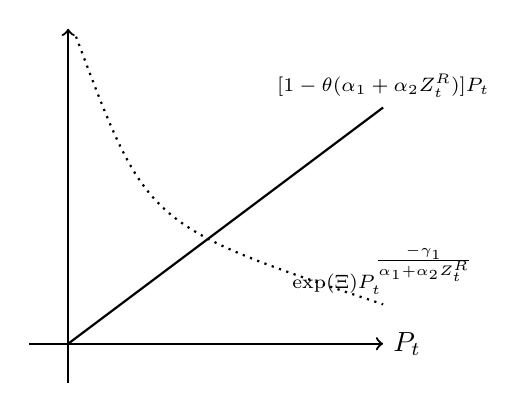
\begin{tikzpicture}
            \draw[->,thick] (-0.5,0)--(4,0) node[right]{$P_t$};
            \draw[->,thick] (0,-0.5)--(0,4) ;
            \draw[dotted, thick] (0.1, 3.9) .. controls (1, 1.5)..(4,0.5) node[above]{\scriptsize{$\exp(\Xi) P_t^{\frac{-\gamma_1}{\alpha_1 + \alpha_2 Z^{R}_{t}}}$}};
            \draw[thick] (0,0) -- (4,3) node[above]{\scriptsize{$[1-\theta(\alpha_1+\alpha_2 Z_t^R)]P_t$}};
        \end{tikzpicture}
        \caption{$\frac{-\gamma_1}{\alpha_1 + \alpha_2 Z^{R}_{t}} < 0$}
        \label{fig:fixed_monotone_decreasing}
    \end{subfigure}
    \hfill
    \begin{subfigure}{0.45\textwidth}
        \begin{tikzpicture}
            \draw[->,thick] (-0.5,0)--(4,0) node[right]{$P_t$};
            \draw[->,thick] (0,-0.5)--(0,4) ;
            \draw[dotted, thick] (0,0) .. controls (1, 2.0)..(4,2.5);
            \draw[thick] (0,0) -- (4,3);
        \end{tikzpicture}
         \caption{$\frac{-\gamma_1}{\alpha_1 + \alpha_2 Z^{R}_{t}} \in [0,1)$}
         \label{fig:fixed_concave}
    \end{subfigure}
    
    \vspace{1em}
    \begin{subfigure}{0.45\textwidth}
        \begin{tikzpicture}
            \draw[->,thick] (-0.5,0)--(4,0) node[right]{$P_t$};
            \draw[->,thick] (0,-0.5)--(0,4) ;
            \draw[dotted, thick] (0,0) -- (4,3);
            \draw[thin] (0,0) -- (4,3);
        \end{tikzpicture}
         \caption{$\frac{-\gamma_1}{\alpha_1 + \alpha_2 Z^{R}_{t}} = 1, 1-\theta(\alpha_1+\alpha_2 Z_t^R) = \exp(\Xi) $}
         \label{fig:fixed_coinside}
    \end{subfigure}
    \hfill
    \begin{subfigure}{0.45\textwidth}
        \begin{tikzpicture}
            \draw[->,thick] (-0.5,0)--(4,0) node[right]{$P_t$};
            \draw[->,thick] (0,-0.5)--(0,4) ;
            \draw[dotted, thick] (0,0) -- (4,3.9);
            \draw[thin] (0,0) -- (4,3);
        \end{tikzpicture}
         \caption{$\frac{-\gamma_1}{\alpha_1 + \alpha_2 Z^{R}_{t}} = 1, 1-\theta(\alpha_1+\alpha_2 Z_t^R) \ne \exp(\Xi) $}
         \label{fig:fixed_parallel}
    \end{subfigure}
    \vspace{1em}
    \begin{subfigure}{0.4\textwidth}
        \begin{tikzpicture}
            \draw[->,thick] (-0.5,0)--(4,0) node[right]{$P_t$};
            \draw[->,thick] (0,-0.5)--(0,4) ;
            \draw[dotted, thick] (0,0) .. controls (2, 0.5)..(4,3.5);
            \draw[thin] (0,0) -- (4,3);
        \end{tikzpicture}
         \caption{$\frac{-\gamma_1}{\alpha_1 + \alpha_2 Z^{R}_{t}}> 1$}
         \label{fig:fixed_convex}
    \end{subfigure}
    
    \footnotesize
    Note: As there is no equilibrium when $1- \theta(\alpha_1 + \alpha_2 Z^{R}_{t}) \le 0$, the above figures assume that $1- \theta(\alpha_1 + \alpha_2 Z^{R}_{t}) > 0$.
    The thick line represents the first term and the dotted line represents the second term in \eqref{eq:fixed_point}.
\end{figure}


From $\Delta (P_t) = 0$, the positive equilibrium price can be written as 
\begin{align}
    0 & = [1-\theta(\alpha_1 + \alpha_2 Z^{R}_{t})]P_t - \exp(\Xi) P_t^{\frac{-\gamma_1}{\alpha_1 + \alpha_2 Z^{R}_{t}}}\nonumber \\ 
    0 & = 1-\theta(\alpha_1 + \alpha_2 Z^{R}_{t}) - \exp(\Xi)P_t^{\frac{-\gamma_1}{\alpha_1 + \alpha_2 Z^{R}_{t}}- 1} \nonumber\\ 
    P_t^{\frac{-\gamma_1}{\alpha_1 + \alpha_2 Z^{R}_{t}}- 1} & = \frac{1-\theta(\alpha_1 + \alpha_2 Z^{R}_{t})}{ \exp(\Xi)}\nonumber\\ 
    P_{t}^* &= \left(\frac{1-\theta(\alpha_1 + \alpha_2 Z^{R}_{t})}{\exp(\Xi)}\right)^{-\frac{\alpha_1 + \alpha_2 Z^{R}_{t}}{\gamma_1 +\alpha_1 + \alpha_2 Z^{R}_{t}}}.
\end{align} 

Figure \ref{fg:equilibrium_existence_demand_supply} illustrates how the demand and supply equations cross under the conditions.
When $1- \theta(\alpha_1 + \alpha_2 Z^{R}_{t}) \le 0$, the supply equation \eqref{eq:log_linear_supply_equation} is ill-defined because the inside of the log function becomes negative.
Thus, there should not be any equilibrium.
Hereafter, assume that $1- \theta(\alpha_1 + \alpha_2 Z^{R}_{t}) > 0$.
When $-\gamma_1/(\alpha_1 + \alpha_2 Z^{R}_{t}) = 1$ and $\exp(\Xi) = 1- \theta(\alpha_1 + \alpha_2 Z^{R}_{t})$, the demand equation and supply equation coincides.
Thus there are infinitely many equilibria in the model.
When $-\gamma_1/(\alpha_1 + \alpha_2 Z^{R}_{t}) = 1$ and $\exp(\Xi) \ne 1- \theta(\alpha_1 + \alpha_2 Z^{R}_{t})$, the demand and supply equations have a same slope and different intercepts, which means that both equations become parallel.
Thus, there is no equilibrium.
When $-\gamma_1/(\alpha_1 + \alpha_2 Z^{R}_{t}) \ne 1$, the demand and supply equations have different slopes, and hence we can find a unique equilibrium. 


\begin{figure}[!ht]
    \caption{The illustrations of the equilibrium existence and uniqueness conditions}
    \label{fg:equilibrium_existence_demand_supply}
    \begin{subfigure}{0.45\textwidth}
        \begin{tikzpicture}
            \draw[->,thick] (-0.5,0)--(4,0) node[right]{$Q_t$};
            \draw[->,thick] (0,-0.5)--(0,4) node[above]{$P_t$};
            \draw[blue, thick] (0,0.5) .. controls (1, 2.2)..(4,3) node[right]{$S$};
            \draw[red, thin] (0,0.5) .. controls (1, 2.2)..(4,3) node[above]{$D$};
        \end{tikzpicture}
         \caption{$-\gamma_1/(\alpha_1 + \alpha_2 Z^{R}_{t}) = 1$ and $\exp(\Xi) = 1- \theta(\alpha_1 + \alpha_2 Z^{R}_{t})$}
    \end{subfigure}
    \hfill
    \begin{subfigure}{0.45\textwidth}
        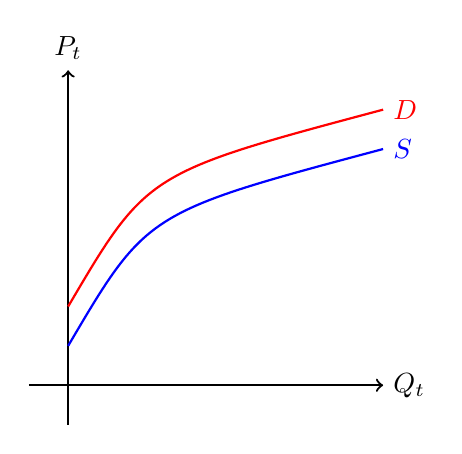
\begin{tikzpicture}
            \draw[->,thick] (-0.5,0)--(4,0) node[right]{$Q_t$};
            \draw[->,thick] (0,-0.5)--(0,4) node[above]{$P_t$};
            \draw[blue, thick] (0, 0.5) .. controls (1, 2.2)..(4,3) node[right]{$S$};
            \draw[red, thick, yshift = 5mm] (0, 0.5) .. controls (1, 2.2)..(4,3) node[right]{$D$};
        \end{tikzpicture}
        \caption{$-\gamma_1/(\alpha_1 + \alpha_2 Z^{R}_{t}) = 1$ and $\exp(\Xi) \ne 1- \theta(\alpha_1 + \alpha_2 Z^{R}_{t})$}
    \end{subfigure}
    
    \vspace{1em}
    \begin{subfigure}{0.45\textwidth}
        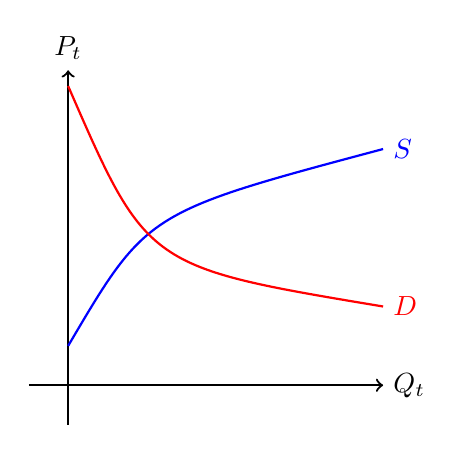
\begin{tikzpicture}
            \draw[->,thick] (-0.5,0)--(4,0) node[right]{$Q_t$};
            \draw[->,thick] (0,-0.5)--(0,4) node[above]{$P_t$};
            \draw[blue, thick] (0,0.5) .. controls (1, 2.2)..(4,3) node[right]{$S$};
            \draw[red, thick] (0,3.8) .. controls (1, 1.5) .. (4,1.0)  node[right]{$D$};
        \end{tikzpicture}
         \caption{$\gamma_1/(\alpha_1 + \alpha_2 Z^{R}_{t}) \ne 1$, $\alpha_1 + \alpha_2 Z^{R}_{t}>0$, and $\gamma_1>0$}
    \end{subfigure}
    \hfill
    \begin{subfigure}{0.45\textwidth}
        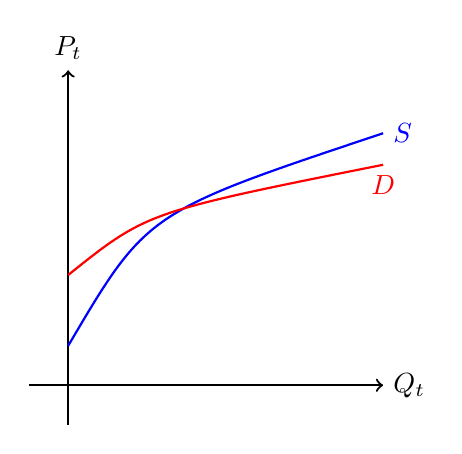
\begin{tikzpicture}
            \draw[->,thick] (-0.5,0)--(4,0) node[right]{$Q_t$};
            \draw[->,thick] (0,-0.5)--(0,4) node[above]{$P_t$};
            \draw[blue, thick] (0,0.5) .. controls (1, 2.2)..(4,3.2) node[right]{$S$};
            \draw[red, thick] (0,1.4) .. controls (1, 2.2) .. (4,2.8)  node[below]{$D$};
        \end{tikzpicture}
         \caption{$\gamma_1/(\alpha_1 + \alpha_2 Z^{R}_{t}) \ne 1$, $\alpha_1 + \alpha_2 Z^{R}_{t}\le0$, and $\gamma_1>0$}
    \end{subfigure}
    \vspace{1em}
    \begin{subfigure}{0.45\textwidth}
        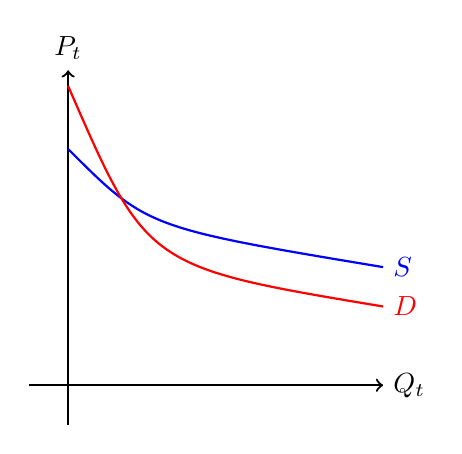
\begin{tikzpicture}
            \draw[->,thick] (-0.5,0)--(4,0) node[right]{$Q_t$};
            \draw[->,thick] (0,-0.5)--(0,4) node[above]{$P_t$};
            \draw[blue, thick] (0,3.0) .. controls (1, 2.0)..(4,1.5) node[right]{$S$};
            \draw[red, thick] (0,3.8) .. controls (1, 1.5) .. (4,1.0)  node[right]{$D$};
        \end{tikzpicture}
         \caption{$\gamma_1/(\alpha_1 + \alpha_2 Z^{R}_{t}) \ne 1$, $\alpha_1 + \alpha_2 Z^{R}_{t}>0$, and $\gamma_1\le 0$}
    \end{subfigure}
    \hfill
    \begin{subfigure}{0.45\textwidth}
        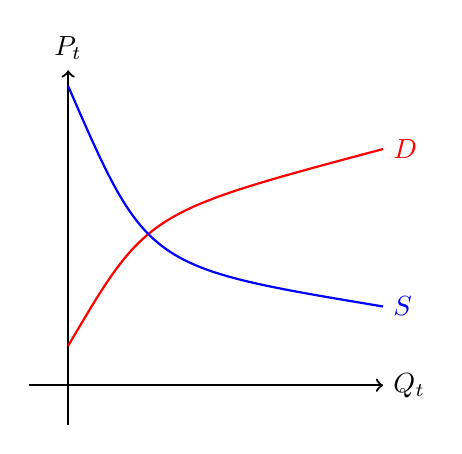
\begin{tikzpicture}
            \draw[->,thick] (-0.5,0)--(4,0) node[right]{$Q_t$};
            \draw[->,thick] (0,-0.5)--(0,4) node[above]{$P_t$};
            \draw[red, thick] (0,0.5) .. controls (1, 2.2)..(4,3) node[right]{$D$};
            \draw[blue, thick] (0,3.8) .. controls (1, 1.5) .. (4,1.0)  node[right]{$S$};
        \end{tikzpicture}
         \caption{$\gamma_1/(\alpha_1 + \alpha_2 Z^{R}_{t}) \ne 1$, $\alpha_1 + \alpha_2 Z^{R}_{t}\le 0$, and $\gamma_1\le 0$}
    \end{subfigure}
    
    \footnotesize
    Note: As there is no equilibrium when $1- \theta(\alpha_1 + \alpha_2 Z^{R}_{t}) \le 0$, the above figures assume that $1- \theta(\alpha_1 + \alpha_2 Z^{R}_{t}) > 0$. 
    %Case (a) considers the case $-\gamma_1/(\alpha_1 + \alpha_2 Z^{R}_{t}) = 1$ and $\exp(\Xi) = 1- \theta(\alpha_1 + \alpha_2 Z^{R}_{t})$. Case (b) considers the case $-\gamma_1/(\alpha_1 + \alpha_2 Z^{R}_{t}) = 1$ and $\exp(\Xi) \ne 1- \theta(\alpha_1 + \alpha_2 Z^{R}_{t})$.
    %Case (c), (d), (e), and (f) consider the case $\gamma_1/(\alpha_1 + \alpha_2 Z^{R}_{t}) \ne 1$.
    Case (a) and (b) also allow both the demand and supply equations to be downward sloping.
\end{figure}







\newpage


\subsection{Simulation and estimation procedure}\label{sec:setting}
To generate the simulation data, for each model, we first generate the exogenous variables $Y_t, Z^{R}_{t}, W_t, R_{t}, H_t$, and $K_t$ and the error terms $\varepsilon_{t}^c$ and $\varepsilon_{t}^d$ based on the data generation process in Table \ref{tb:parameter_setting}.
By substituting the Equation \eqref{eq:log_linear_demand} into Equation \eqref{eq:log_linear_supply_equation} and solving it for $P_{t}$, the log aggregate quantity is given as: 
\begin{align}
    \log Q_t &= \frac{ \alpha_0 + \alpha_3 \log Y_t + \log (1 - \theta (\alpha_1 + \alpha_2 Z^{R}_{t})) - \gamma_0  -  \gamma_2 \log W_{t} - \gamma_3 \log R_t + \varepsilon^{d}_{t} - \varepsilon^{c}_{t}}{\gamma_1+ \alpha_1 + \alpha_2 Z^{R}_{t} }.\label{eq:quantity_loglinear}
\end{align}
We compute the equilibrium quantity $Q_{t}$ for the log-linear model by \eqref{eq:quantity_loglinear}.
We then compute the equilibrium price $P_t$ by substituting $Q_{t}$ and other variables into the demand function \eqref{eq:log_linear_demand}.
We generate 1000 data sets of 100, 200, 1000, 1500 markets.
We jointly estimate the demand and supply parameters by the simultaneous equation model \citep{wooldridge2010econometric} from the true values.
We use state-of-the-art constrained optimization solvers, i.e., \texttt{Ipopt.jl} which implements an interior point line search filter method that aims to find a local solution of nonlinear programming problems.



\begin{table}[!htbp]
    \caption{True parameters and distributions}
    \label{tb:parameter_setting}
    \begin{center}
    \subfloat[Parameters]{
    \begin{tabular}{crr}
            \hline
            $\alpha_0$  & $20.0$ &\\
            $\alpha_1$ & $1.0$  &\\
            $\alpha_2$ & $0.1$ &\\
            $\alpha_3$ & $1.0$ &\\
            $\gamma_0$ & $5.0$  &\\
            $\gamma_1$ & $1.0$  &\\
            $\gamma_2$ & $1.0$ &\\
            $\gamma_3$ & $1.0$ &\\
            $\theta$ & $0.5$  &\\
            \hline
        \end{tabular}
    }
    \subfloat[Distributions]{
    \begin{tabular}{crr}
            \hline
            Demand shifter&  &  \\
            $Y_t$ & $N(0,1)$ \\
            Demand rotation instrument&  &  \\
            $Z^{R}_{t}$ & $U(0,1)$ \\
            Cost shifter  &  \\
            $W_{t}$ & $U(1,3)$ \\
            $R_t$  & $U(1,3)$  \\
            $H_{t}$ & $W_{t}+U(0,1)$  \\
            $K_{t}$ & $R_{t}+U(0,1)$  \\
            Error&  &  \\
            $\varepsilon^{d}_{t}$ & $N(0,\sigma)$  \\
            $\varepsilon^{c}_{t}$ & $N(0,\sigma)$ \\
            \hline
        \end{tabular}
    }
    \end{center}
    \footnotesize
    Note: $\sigma=\{0.5, 1.0, 2.0\}$. $N:$ Normal distribution. $U:$ Uniform distribution.
\end{table}

\subsection{Why does the estimation without equilibrium conditions converge to the extremely low conduct parameters?}

We should interpret reasons why the estimation without equilibrium conditions converges to the negative conduct parameters, as shown in Panel (a) in Table \ref{tb:loglinear_loglinear_sigma_1_simultaneous_non_constraint_theta_constraint_bias_rmse}, although the obtained parameters cannot be interpreted as the exogenous elements determining equilibrium outcomes. 
First, we rewrite the terms in Equation \eqref{eq:residual_supply_2sls} into $$\log(1 - \theta C_{t})-\gamma_{0}$$
where $C_{t}=\alpha_1 + \alpha_2 Z^{R}_{t}$ is given in the demand estimation.
If the model allows $\theta<0$, then $1 - \theta C_{t}$ can take an arbitrarily large value through log-transformation relative to $\gamma_0$. 
For example, if $1 - \theta C_{t}=1,000,000$, then $\log(1 - \theta C_{t})=13.8$, which has a small contribution relative to $\gamma_0$ for evaluating the moment conditions.

% \footnote{The expansion of $\log(1+x)$ around $x=0$ is given by: $\log(1+x) = x - (x^2)/2 + (x^3)/3 - (x^4)/4 + \cdots$. This is known as the Taylor series expansion of the natural logarithm function around $x=0$.} The second order Taylor expansion around $\theta=0$ is 
% $$\log(1 - \theta(\alpha_1 + \alpha_2 Z^{R}_{t}))-\gamma_{0}\approx -\theta(\alpha_1 + \alpha_2 Z^{R}_{t}) - \frac{(-\theta(\alpha_1 + \alpha_2 Z^{R}_{t}))^2}{2}-\gamma_{0}$$




\subsection{Additional experiments}\label{sec:additional_experiments}

Additional results for different $\sigma$ are shown in Tables \ref{tb:loglinear_loglinear_sigma_0.5_simultaneous_theta_constraint_slope_constraint_bias_rmse} and \ref{tb:loglinear_loglinear_sigma_2_simultaneous_theta_constraint_non_constraint_bias_rmse}. 
As a summary, the main findings in the main text are robust.

In Tables \ref{tb:linear_linear_sigma_1} and  \ref{tb:linear_linear_sigma_2_mpec_linear_non_constraint_theta_constraint_bias_rmse}, we illustrate that N2SLS with Constraints \eqref{eq:conduct_constraint} works for the linear model as in \cite{matsumura2023resolving}. 
This means that incorporating the conditions is innocuous for the linear model.

Additional ad hoc improvement is possible by using \eqref{eq:log_linear_marginal_cost} to compute $\varepsilon_t^c$ and \eqref{eq:log_linear_supply_equation_direct} as constraints with Constraints \eqref{eq:conduct_constraint}, \eqref{eq:slope_constraint}, and \eqref{eq:equlibrium_existence}. 
Table \ref{tb:loglinear_loglinear_sigma_2_mpec_theta_constraint_non_constraint_bias_rmse} shows that the estimation of the conduct parameter $\theta$ improves, that is, the bias is 0.014 and RMSE is 0.217. 
However, the results with ad hoc improvement do not dominate the results without the improvement for all parameters.

\begin{landscape}{
\begin{table}[!htbp]
  \begin{center}
      \caption{Performance comparison ($\sigma=0.5$)}
      \label{tb:loglinear_loglinear_sigma_0.5_simultaneous_theta_constraint_slope_constraint_bias_rmse} 
      \subfloat[N2SLS without Constraints \eqref{eq:conduct_constraint}, \eqref{eq:slope_constraint}, and \eqref{eq:equlibrium_existence}]{
\begin{tabular}[t]{llrrrrrrr}
\toprule
  & Bias & RMSE & Bias & RMSE & Bias & RMSE & Bias & RMSE\\
\midrule
$\alpha_{0}$ & 0.715 & 0.815 & 0.765 & 0.797 & 0.788 & 0.804 & 0.795 & 0.797\\
$\alpha_{1}$ & -0.169 & 0.900 & -0.066 & 0.514 & -0.018 & 0.337 & 0.005 & 0.118\\
$\alpha_{2}$ & -0.039 & 0.379 & -0.019 & 0.223 & -0.011 & 0.153 & -0.016 & 0.077\\
$\alpha_{3}$ & 0.707 & 1.047 & 0.794 & 0.941 & 0.834 & 0.900 & 0.855 & 0.864\\
$\gamma_{0}$ & 3.128 & 4.732 & 2.932 & 4.511 & 2.626 & 4.151 & 1.473 & 3.022\\
$\gamma_{1}$ & 0.040 & 0.302 & 0.015 & 0.194 & 0.005 & 0.130 & -0.001 & 0.056\\
$\gamma_{2}$ & 0.007 & 0.299 & 0.009 & 0.195 & 0.005 & 0.130 & 0.000 & 0.059\\
$\gamma_{3}$ & 0.018 & 0.173 & 0.008 & 0.110 & 0.002 & 0.075 & -0.001 & 0.033\\
$\theta$ & -1767.327 & 6217.525 & -1024.935 & 2976.989 & -751.215 & 2765.357 & -240.693 & 974.357\\
Runs converged (\%) &  & 99.000 &  & 98.500 &  & 99.100 &  & 98.700\\
Sample size ($T$) &  & 50 &  & 100 &  & 200 &  & 1000\\
\bottomrule
\end{tabular}
}\\
    \subfloat[N2SLS with Constraints \eqref{eq:conduct_constraint}, \eqref{eq:slope_constraint}, and \eqref{eq:equlibrium_existence}]{
\begin{tabular}[t]{lrrrrrrrr}
\toprule
  & Bias & RMSE & Bias & RMSE & Bias & RMSE & Bias & RMSE\\
\midrule
$\alpha_{0}$ & -0.006 & 3.556 & 0.175 & 3.158 & 0.059 & 0.977 & -0.017 & 0.763\\
$\alpha_{1}$ & -0.002 & 0.545 & 0.026 & 0.484 & 0.009 & 0.150 & -0.003 & 0.117\\
$\alpha_{2}$ & 0.002 & 0.044 & 0.004 & 0.037 & 0.000 & 0.012 & 0.000 & 0.010\\
$\alpha_{3}$ & 0.001 & 0.309 & 0.012 & 0.266 & 0.005 & 0.091 & 0.000 & 0.073\\
$\gamma_{0}$ & -0.616 & 3.317 & -0.221 & 2.191 & 0.275 & 1.076 & 0.421 & 0.972\\
$\gamma_{1}$ & 0.089 & 0.399 & 0.038 & 0.252 & -0.015 & 0.107 & -0.027 & 0.089\\
$\gamma_{2}$ & 0.044 & 0.265 & 0.022 & 0.170 & -0.007 & 0.074 & -0.011 & 0.061\\
$\gamma_{3}$ & 0.046 & 0.273 & 0.019 & 0.178 & -0.008 & 0.078 & -0.012 & 0.059\\
$\theta$ & -0.064 & 0.390 & -0.079 & 0.339 & -0.119 & 0.260 & -0.145 & 0.261\\
Runs converged (\%) &  & 99.900 &  & 100.000 &  & 100.000 &  & 100.000\\
Sample size ($T$) &  & 100 &  & 200 &  & 1000 &  & 1500\\
\bottomrule
\end{tabular}
}
  \end{center}
  \footnotesize
  
\end{table} 
}
\end{landscape}

\begin{landscape}{
\begin{table}[!htbp]
  \begin{center}
      \caption{Performance comparison ($\sigma=2.0$)}
      \label{tb:loglinear_loglinear_sigma_2_simultaneous_theta_constraint_non_constraint_bias_rmse} 
      \subfloat[N2SLS without Constraints \eqref{eq:conduct_constraint}, \eqref{eq:slope_constraint}, and \eqref{eq:equlibrium_existence}]{
\begin{tabular}[t]{llrrrrrrr}
\toprule
  & Bias & RMSE & Bias & RMSE & Bias & RMSE & Bias & RMSE\\
\midrule
$\alpha_{0}$ & -3.378 & 8.412 & -2.417 & 11.769 & -1.420 & 8.994 & 0.251 & 5.398\\
$\alpha_{1}$ & -0.497 & 1.238 & -0.357 & 1.780 & -0.214 & 1.314 & 0.056 & 1.011\\
$\alpha_{2}$ & -0.032 & 0.182 & -0.018 & 0.130 & -0.009 & 0.128 & 0.003 & 0.060\\
$\alpha_{3}$ & -0.278 & 1.239 & -0.176 & 0.970 & -0.136 & 0.870 & 0.004 & 0.446\\
$\gamma_{0}$ & 8.326 & 19.286 & 8.722 & 24.643 & 10.222 & 13.821 & 12.193 & 12.555\\
$\gamma_{1}$ & -0.055 & 2.271 & 0.056 & 3.006 & -0.090 & 1.170 & -0.132 & 0.390\\
$\gamma_{2}$ & -0.133 & 2.091 & -0.008 & 1.880 & -0.061 & 0.758 & -0.055 & 0.278\\
$\gamma_{3}$ & -0.108 & 1.796 & 0.019 & 2.235 & -0.042 & 0.830 & -0.064 & 0.281\\
$\theta$ & -3954520.714 & 84084952.193 & -596779.310 & 3976692.924 & -369662.580 & 2175356.919 & -111842.897 & 159200.718\\
Runs converged (\%) &  & 99.700 &  & 99.800 &  & 99.900 &  & 98.000\\
Sample size ($T$) &  & 50 &  & 100 &  & 200 &  & 1000\\
\bottomrule
\end{tabular}
}\\
    \subfloat[N2SLS with Constraints \eqref{eq:conduct_constraint}, \eqref{eq:slope_constraint}, and \eqref{eq:equlibrium_existence}]{
\begin{tabular}[t]{llrrrrrrr}
\toprule
  & Bias & RMSE & Bias & RMSE & Bias & RMSE & Bias & RMSE\\
\midrule
$\alpha_{0}$ & -2.022 & 11.280 & -1.149 & 8.680 & 0.138 & 4.651 & 0.274 & 3.838\\
$\alpha_{1}$ & -0.310 & 1.771 & -0.181 & 1.313 & 0.019 & 0.712 & 0.041 & 0.590\\
$\alpha_{2}$ & -0.016 & 0.136 & -0.007 & 0.139 & 0.003 & 0.057 & 0.004 & 0.043\\
$\alpha_{3}$ & -0.148 & 0.984 & -0.113 & 0.875 & -0.003 & 0.428 & 0.017 & 0.333\\
$\gamma_{0}$ & 0.672 & 11.896 & -1.090 & 13.475 & -0.669 & 4.499 & -0.404 & 3.245\\
$\gamma_{1}$ & -0.046 & 1.598 & 0.172 & 1.770 & 0.098 & 0.556 & 0.066 & 0.391\\
$\gamma_{2}$ & -0.057 & 1.085 & 0.088 & 1.172 & 0.054 & 0.346 & 0.024 & 0.252\\
$\gamma_{3}$ & -0.020 & 1.204 & 0.108 & 1.225 & 0.050 & 0.365 & 0.031 & 0.267\\
$\theta$ & -0.229 & 0.475 & -0.163 & 0.464 & -0.088 & 0.410 & -0.108 & 0.394\\
Runs converged (\%) &  & 99.500 &  & 99.200 &  & 100.000 &  & 100.000\\
Sample size ($T$) &  & 100 &  & 200 &  & 1000 &  & 1500\\
\bottomrule
\end{tabular}
}
  \end{center}
  \footnotesize
  
\end{table} 
}
\end{landscape}


\begin{table}[!htbp]
  \begin{center}
      \caption{Ad hoc method using \eqref{eq:log_linear_marginal_cost} to compute $\varepsilon_t^c$ and \eqref{eq:log_linear_supply_equation_direct} as constraints with  Constraints \eqref{eq:conduct_constraint}, \eqref{eq:slope_constraint}, and \eqref{eq:equlibrium_existence}}
      \label{tb:loglinear_loglinear_sigma_2_mpec_theta_constraint_non_constraint_bias_rmse} 
      \subfloat[$\sigma=0.5$]{
\begin{tabular}[t]{llrrrrrrr}
\toprule
  & Bias & RMSE & Bias & RMSE & Bias & RMSE & Bias & RMSE\\
\midrule
$\alpha_{0}$ & -0.347 & 2.978 & -0.153 & 2.547 & 0.065 & 0.976 & -0.009 & 0.760\\
$\alpha_{1}$ & -0.043 & 0.452 & -0.016 & 0.388 & 0.010 & 0.150 & -0.001 & 0.117\\
$\alpha_{2}$ & -0.024 & 0.065 & -0.017 & 0.054 & 0.000 & 0.012 & 0.000 & 0.010\\
$\alpha_{3}$ & -0.028 & 0.265 & -0.013 & 0.224 & 0.005 & 0.091 & 0.001 & 0.073\\
$\gamma_{0}$ & -2.458 & 5.660 & -1.258 & 2.959 & -0.132 & 0.942 & -0.153 & 0.748\\
$\gamma_{1}$ & 0.112 & 0.602 & 0.057 & 0.260 & 0.014 & 0.103 & 0.014 & 0.082\\
$\gamma_{2}$ & 0.053 & 0.314 & 0.030 & 0.172 & 0.007 & 0.073 & 0.010 & 0.060\\
$\gamma_{3}$ & 0.061 & 0.426 & 0.028 & 0.181 & 0.006 & 0.077 & 0.008 & 0.058\\
$\theta$ & 0.169 & 0.407 & 0.109 & 0.356 & -0.003 & 0.155 & 0.017 & 0.116\\
Runs converged (\%) &  & 100.000 &  & 100.000 &  & 100.000 &  & 100.000\\
Sample size ($T$) &  & 100 &  & 200 &  & 1000 &  & 1500\\
\bottomrule
\end{tabular}
}\\
      \subfloat[$\sigma=1.0$]{
\begin{tabular}[t]{lrrrrrrrr}
\toprule
  & Bias & RMSE & Bias & RMSE & Bias & RMSE & Bias & RMSE\\
\midrule
$\alpha_{0}$ & -0.614 & 5.995 & -0.213 & 4.315 & 0.077 & 2.034 & 0.063 & 1.555\\
$\alpha_{1}$ & -0.085 & 0.902 & -0.024 & 0.663 & 0.011 & 0.312 & 0.010 & 0.240\\
$\alpha_{2}$ & -0.028 & 0.105 & -0.022 & 0.073 & 0.000 & 0.025 & 0.001 & 0.020\\
$\alpha_{3}$ & -0.070 & 0.549 & -0.019 & 0.431 & -0.001 & 0.185 & 0.004 & 0.152\\
$\gamma_{0}$ & -5.106 & 15.922 & -2.379 & 6.990 & -0.375 & 1.959 & -0.398 & 1.533\\
$\gamma_{1}$ & 0.386 & 2.047 & 0.141 & 0.839 & 0.045 & 0.229 & 0.044 & 0.175\\
$\gamma_{2}$ & 0.190 & 1.155 & 0.054 & 0.475 & 0.022 & 0.150 & 0.027 & 0.120\\
$\gamma_{3}$ & 0.163 & 1.006 & 0.065 & 0.482 & 0.013 & 0.149 & 0.023 & 0.121\\
$\theta$ & 0.186 & 0.442 & 0.158 & 0.422 & -0.007 & 0.275 & 0.014 & 0.217\\
Runs converged (\%) &  & 100.000 &  & 100.000 &  & 100.000 &  & 100.000\\
Sample size ($T$) &  & 100 &  & 200 &  & 1000 &  & 1500\\
\bottomrule
\end{tabular}
}\\
      \subfloat[$\sigma=2.0$]{
\begin{tabular}[t]{lrrrrrrrr}
\toprule
  & Bias & RMSE & Bias & RMSE & Bias & RMSE & Bias & RMSE\\
\midrule
$\alpha_{0}$ & -0.835 & 9.908 & -0.561 & 6.310 & 0.147 & 4.424 & 0.301 & 3.686\\
$\alpha_{1}$ & -0.109 & 1.563 & -0.076 & 0.935 & 0.024 & 0.677 & 0.047 & 0.566\\
$\alpha_{2}$ & -0.043 & 0.124 & -0.033 & 0.135 & -0.005 & 0.061 & 0.001 & 0.045\\
$\alpha_{3}$ & -0.047 & 0.909 & -0.078 & 0.664 & -0.004 & 0.404 & 0.018 & 0.323\\
$\gamma_{0}$ & -6.629 & 20.418 & -5.373 & 16.692 & -1.445 & 4.738 & -1.123 & 3.411\\
$\gamma_{1}$ & 0.422 & 2.630 & 0.384 & 2.103 & 0.137 & 0.580 & 0.115 & 0.409\\
$\gamma_{2}$ & 0.184 & 1.788 & 0.185 & 1.318 & 0.073 & 0.357 & 0.048 & 0.261\\
$\gamma_{3}$ & 0.199 & 1.885 & 0.215 & 1.496 & 0.068 & 0.376 & 0.055 & 0.276\\
$\theta$ & 0.225 & 0.459 & 0.227 & 0.447 & 0.098 & 0.357 & 0.084 & 0.313\\
Runs converged (\%) &  & 99.200 &  & 99.800 &  & 99.800 &  & 100.000\\
Sample size ($T$) &  & 100 &  & 200 &  & 1000 &  & 1500\\
\bottomrule
\end{tabular}
}
  \end{center}
  \footnotesize
  
\end{table} 




\begin{table}[!htbp]
  \begin{center}
      \caption{N2SLS without Constraints \eqref{eq:conduct_constraint} Results of the linear model}
      \label{tb:linear_linear_sigma_1} 
      \subfloat[$\sigma=0.5$]{
\begin{tabular}[t]{llrrrrrrr}
\toprule
  & Bias & RMSE & Bias & RMSE & Bias & RMSE & Bias & RMSE\\
\midrule
$\alpha_{0}$ & -0.018 & 0.465 & 0.007 & 0.323 & -0.008 & 0.213 & -0.006 & 0.097\\
$\alpha_{1}$ & -0.045 & 2.257 & 0.024 & 1.523 & 0.018 & 1.016 & -0.031 & 0.455\\
$\alpha_{2}$ & -0.001 & 0.255 & -0.001 & 0.176 & -0.004 & 0.115 & 0.001 & 0.051\\
$\alpha_{3}$ & -0.005 & 0.108 & 0.003 & 0.075 & -0.001 & 0.050 & -0.001 & 0.022\\
$\gamma_{0}$ & -0.061 & 0.732 & -0.005 & 0.474 & -0.021 & 0.346 & -0.005 & 0.152\\
$\gamma_{1}$ & -0.311 & 3.450 & -0.124 & 1.928 & -0.081 & 1.303 & -0.003 & 0.548\\
$\gamma_{2}$ & 0.009 & 0.109 & -0.001 & 0.071 & 0.003 & 0.051 & 0.000 & 0.023\\
$\gamma_{3}$ & 0.001 & 0.108 & 0.003 & 0.075 & 0.003 & 0.053 & 0.000 & 0.022\\
$\theta$ & 0.047 & 0.354 & 0.017 & 0.209 & 0.014 & 0.135 & 0.003 & 0.058\\
Sample size (n) &  & 50 &  & 100 &  & 200 &  & 1000\\
\bottomrule
\end{tabular}
}\\
      \subfloat[$\sigma=1.0$]{
\begin{tabular}[t]{llrrrrrrr}
\toprule
  & Bias & RMSE & Bias & RMSE & Bias & RMSE & Bias & RMSE\\
\midrule
$\alpha_{0}$ & -0.027 & 1.023 & -0.002 & 0.641 & -0.004 & 0.448 & -0.016 & 0.188\\
$\alpha_{1}$ & -0.024 & 4.396 & -0.169 & 2.965 & 0.061 & 2.060 & 0.011 & 0.905\\
$\alpha_{2}$ & -0.006 & 0.494 & 0.016 & 0.325 & -0.007 & 0.234 & -0.006 & 0.100\\
$\alpha_{3}$ & -0.006 & 0.223 & 0.002 & 0.153 & -0.001 & 0.099 & -0.003 & 0.045\\
$\gamma_{0}$ & -0.318 & 1.769 & -0.091 & 1.059 & -0.086 & 0.714 & -0.004 & 0.308\\
$\gamma_{1}$ & 5.859 & 210.853 & -0.679 & 6.280 & -0.338 & 2.972 & -0.050 & 1.110\\
$\gamma_{2}$ & 0.035 & 0.247 & 0.011 & 0.157 & 0.011 & 0.104 & 0.000 & 0.045\\
$\gamma_{3}$ & 0.045 & 0.250 & 0.012 & 0.150 & 0.010 & 0.104 & 0.002 & 0.045\\
$\theta$ & -0.399 & 18.450 & 0.098 & 0.738 & 0.054 & 0.308 & 0.009 & 0.113\\
Sample size (n) &  & 50 &  & 100 &  & 200 &  & 1000\\
\bottomrule
\end{tabular}
}\\
    \subfloat[$\sigma=2.0$]{
\begin{tabular}[t]{llrrrrrrr}
\toprule
  & Bias & RMSE & Bias & RMSE & Bias & RMSE & Bias & RMSE\\
\midrule
$\alpha_{0}$ & -0.263 & 2.596 & 0.071 & 1.670 & -0.040 & 0.947 & -0.002 & 0.412\\
$\alpha_{1}$ & -0.271 & 10.820 & 0.008 & 6.492 & 0.236 & 4.263 & 0.021 & 1.809\\
$\alpha_{2}$ & -0.044 & 1.253 & 0.023 & 0.779 & -0.031 & 0.483 & -0.003 & 0.210\\
$\alpha_{3}$ & -0.024 & 0.584 & 0.008 & 0.343 & -0.004 & 0.225 & 0.003 & 0.092\\
$\gamma_{0}$ & -2.074 & 19.624 & -0.551 & 3.043 & -0.171 & 1.516 & -0.051 & 0.633\\
$\gamma_{1}$ & 58.209 & 1750.688 & -2.416 & 56.909 & -3.617 & 39.044 & -0.103 & 2.334\\
$\gamma_{2}$ & 0.242 & 2.430 & 0.065 & 0.409 & 0.020 & 0.220 & 0.006 & 0.093\\
$\gamma_{3}$ & 0.230 & 2.328 & 0.055 & 0.404 & 0.010 & 0.219 & 0.008 & 0.092\\
$\theta$ & -6.668 & 233.851 & 0.372 & 6.334 & 0.418 & 3.820 & 0.024 & 0.245\\
Sample size ($T$) &  & 50 &  & 100 &  & 200 &  & 1000\\
\bottomrule
\end{tabular}
}
  \end{center}
  \footnotesize
  Note: The data generating process follows \cite{matsumura2023resolving}.
\end{table} 

\begin{table}[!htbp]
  \begin{center}
      \caption{N2SLS with Constraints \eqref{eq:conduct_constraint} for the linear model}
      \label{tb:linear_linear_sigma_2_mpec_linear_non_constraint_theta_constraint_bias_rmse} 
      \subfloat[$\sigma=0.5$]{
\begin{tabular}[t]{llrrrrrrr}
\toprule
  & Bias & RMSE & Bias & RMSE & Bias & RMSE & Bias & RMSE\\
\midrule
$\alpha_{0}$ & -0.013 & 0.462 & 0.008 & 0.322 & -0.008 & 0.213 & -0.006 & 0.097\\
$\alpha_{1}$ & -0.096 & 2.201 & 0.015 & 1.511 & 0.018 & 1.016 & -0.031 & 0.455\\
$\alpha_{2}$ & 0.006 & 0.247 & 0.001 & 0.174 & -0.004 & 0.115 & 0.001 & 0.051\\
$\alpha_{3}$ & -0.004 & 0.108 & 0.003 & 0.074 & -0.001 & 0.050 & -0.001 & 0.022\\
$\gamma_{0}$ & -0.054 & 0.724 & -0.002 & 0.472 & -0.021 & 0.346 & -0.005 & 0.152\\
$\gamma_{1}$ & -0.098 & 2.620 & -0.093 & 1.847 & -0.081 & 1.303 & -0.003 & 0.548\\
$\gamma_{2}$ & 0.008 & 0.108 & -0.002 & 0.070 & 0.003 & 0.051 & 0.000 & 0.023\\
$\gamma_{3}$ & 0.001 & 0.107 & 0.003 & 0.075 & 0.003 & 0.053 & 0.000 & 0.022\\
$\theta$ & 0.023 & 0.258 & 0.014 & 0.197 & 0.014 & 0.135 & 0.003 & 0.058\\
Sample size ($T$) &  & 50 &  & 100 &  & 200 &  & 1000\\
\bottomrule
\end{tabular}
}\\
      \subfloat[$\sigma=1.0$]{
\begin{tabular}[t]{llrrrrrrr}
\toprule
  & Bias & RMSE & Bias & RMSE & Bias & RMSE & Bias & RMSE\\
\midrule
$\alpha_{0}$ & 0.012 & 1.015 & 0.012 & 0.636 & 0.001 & 0.446 & -0.016 & 0.188\\
$\alpha_{1}$ & -0.383 & 4.216 & -0.291 & 2.872 & 0.015 & 2.012 & 0.011 & 0.905\\
$\alpha_{2}$ & 0.042 & 0.466 & 0.033 & 0.310 & -0.001 & 0.227 & -0.006 & 0.100\\
$\alpha_{3}$ & 0.000 & 0.222 & 0.004 & 0.152 & 0.000 & 0.099 & -0.003 & 0.045\\
$\gamma_{0}$ & -0.233 & 1.612 & -0.067 & 1.020 & -0.076 & 0.703 & -0.004 & 0.308\\
$\gamma_{1}$ & 0.406 & 4.332 & -0.024 & 3.174 & -0.178 & 2.585 & -0.050 & 1.110\\
$\gamma_{2}$ & 0.025 & 0.231 & 0.008 & 0.154 & 0.010 & 0.103 & 0.000 & 0.045\\
$\gamma_{3}$ & 0.034 & 0.233 & 0.010 & 0.146 & 0.009 & 0.103 & 0.002 & 0.045\\
$\theta$ & 0.014 & 0.380 & 0.018 & 0.311 & 0.035 & 0.260 & 0.009 & 0.113\\
Sample size ($T$) &  & 50 &  & 100 &  & 200 &  & 1000\\
\bottomrule
\end{tabular}
}\\
    \subfloat[$\sigma=2.0$]{
\begin{tabular}[t]{llrrrrrrr}
\toprule
  & Bias & RMSE & Bias & RMSE & Bias & RMSE & Bias & RMSE\\
\midrule
$\alpha_{0}$ & -0.138 & 2.592 & 0.142 & 1.671 & 0.004 & 0.936 & 0.000 & 0.410\\
$\alpha_{1}$ & -0.986 & 11.090 & -0.665 & 6.325 & -0.174 & 4.042 & 0.003 & 1.788\\
$\alpha_{2}$ & 0.065 & 1.255 & 0.112 & 0.756 & 0.023 & 0.447 & 0.000 & 0.207\\
$\alpha_{3}$ & -0.006 & 0.589 & 0.019 & 0.345 & 0.003 & 0.224 & 0.003 & 0.092\\
$\gamma_{0}$ & -0.123 & 3.350 & -0.298 & 2.455 & -0.081 & 1.379 & -0.047 & 0.628\\
$\gamma_{1}$ & 0.635 & 7.424 & 0.141 & 5.668 & -0.081 & 4.255 & -0.040 & 2.159\\
$\gamma_{2}$ & 0.016 & 0.484 & 0.037 & 0.349 & 0.009 & 0.205 & 0.005 & 0.093\\
$\gamma_{3}$ & 0.009 & 0.517 & 0.026 & 0.336 & 0.000 & 0.208 & 0.007 & 0.092\\
$\theta$ & -0.029 & 0.446 & 0.025 & 0.414 & 0.034 & 0.381 & 0.016 & 0.220\\
Sample size ($T$) &  & 50 &  & 100 &  & 200 &  & 1000\\
\bottomrule
\end{tabular}
}
  \end{center}
  \footnotesize
  Note: The data generating process follows \cite{matsumura2023resolving}.
\end{table} 


% \begin{table}[!htbp]
%   \begin{center}
%       \caption{Additional improvement by adding supply constraints}
%       \label{tb:loglinear_loglinear_sigma_1_mpec_theta_constraint_slope_constraint_bias_rmse} 
%       \subfloat[N2SLS with Constraints \eqref{eq:conduct_constraint}, \eqref{eq:slope_constraint}, \eqref{eq:equlibrium_existence}, and supply constraints ($\sigma=0.5$)]{
\begin{tabular}[t]{llrrrrrrr}
\toprule
  & Bias & RMSE & Bias & RMSE & Bias & RMSE & Bias & RMSE\\
\midrule
$\alpha_{0}$ & -0.347 & 2.978 & -0.153 & 2.547 & 0.065 & 0.976 & -0.009 & 0.760\\
$\alpha_{1}$ & -0.043 & 0.452 & -0.016 & 0.388 & 0.010 & 0.150 & -0.001 & 0.117\\
$\alpha_{2}$ & -0.024 & 0.065 & -0.017 & 0.054 & 0.000 & 0.012 & 0.000 & 0.010\\
$\alpha_{3}$ & -0.028 & 0.265 & -0.013 & 0.224 & 0.005 & 0.091 & 0.001 & 0.073\\
$\gamma_{0}$ & -2.458 & 5.660 & -1.258 & 2.959 & -0.132 & 0.942 & -0.153 & 0.748\\
$\gamma_{1}$ & 0.112 & 0.602 & 0.057 & 0.260 & 0.014 & 0.103 & 0.014 & 0.082\\
$\gamma_{2}$ & 0.053 & 0.314 & 0.030 & 0.172 & 0.007 & 0.073 & 0.010 & 0.060\\
$\gamma_{3}$ & 0.061 & 0.426 & 0.028 & 0.181 & 0.006 & 0.077 & 0.008 & 0.058\\
$\theta$ & 0.169 & 0.407 & 0.109 & 0.356 & -0.003 & 0.155 & 0.017 & 0.116\\
Runs converged (\%) &  & 100.000 &  & 100.000 &  & 100.000 &  & 100.000\\
Sample size ($T$) &  & 100 &  & 200 &  & 1000 &  & 1500\\
\bottomrule
\end{tabular}
}\\
%       \subfloat[N2SLS with Constraints \eqref{eq:conduct_constraint}, \eqref{eq:slope_constraint}, \eqref{eq:equlibrium_existence}, and supply constraints ($\sigma=1.0$)]{
\begin{tabular}[t]{lrrrrrrrr}
\toprule
  & Bias & RMSE & Bias & RMSE & Bias & RMSE & Bias & RMSE\\
\midrule
$\alpha_{0}$ & -0.614 & 5.995 & -0.213 & 4.315 & 0.077 & 2.034 & 0.063 & 1.555\\
$\alpha_{1}$ & -0.085 & 0.902 & -0.024 & 0.663 & 0.011 & 0.312 & 0.010 & 0.240\\
$\alpha_{2}$ & -0.028 & 0.105 & -0.022 & 0.073 & 0.000 & 0.025 & 0.001 & 0.020\\
$\alpha_{3}$ & -0.070 & 0.549 & -0.019 & 0.431 & -0.001 & 0.185 & 0.004 & 0.152\\
$\gamma_{0}$ & -5.106 & 15.922 & -2.379 & 6.990 & -0.375 & 1.959 & -0.398 & 1.533\\
$\gamma_{1}$ & 0.386 & 2.047 & 0.141 & 0.839 & 0.045 & 0.229 & 0.044 & 0.175\\
$\gamma_{2}$ & 0.190 & 1.155 & 0.054 & 0.475 & 0.022 & 0.150 & 0.027 & 0.120\\
$\gamma_{3}$ & 0.163 & 1.006 & 0.065 & 0.482 & 0.013 & 0.149 & 0.023 & 0.121\\
$\theta$ & 0.186 & 0.442 & 0.158 & 0.422 & -0.007 & 0.275 & 0.014 & 0.217\\
Runs converged (\%) &  & 100.000 &  & 100.000 &  & 100.000 &  & 100.000\\
Sample size ($T$) &  & 100 &  & 200 &  & 1000 &  & 1500\\
\bottomrule
\end{tabular}
}\\
%       \subfloat[N2SLS with Constraints \eqref{eq:conduct_constraint}, \eqref{eq:slope_constraint}, \eqref{eq:equlibrium_existence}, and supply constraints ($\sigma=2.0$)]{
\begin{tabular}[t]{lrrrrrrrr}
\toprule
  & Bias & RMSE & Bias & RMSE & Bias & RMSE & Bias & RMSE\\
\midrule
$\alpha_{0}$ & -0.835 & 9.908 & -0.561 & 6.310 & 0.147 & 4.424 & 0.301 & 3.686\\
$\alpha_{1}$ & -0.109 & 1.563 & -0.076 & 0.935 & 0.024 & 0.677 & 0.047 & 0.566\\
$\alpha_{2}$ & -0.043 & 0.124 & -0.033 & 0.135 & -0.005 & 0.061 & 0.001 & 0.045\\
$\alpha_{3}$ & -0.047 & 0.909 & -0.078 & 0.664 & -0.004 & 0.404 & 0.018 & 0.323\\
$\gamma_{0}$ & -6.629 & 20.418 & -5.373 & 16.692 & -1.445 & 4.738 & -1.123 & 3.411\\
$\gamma_{1}$ & 0.422 & 2.630 & 0.384 & 2.103 & 0.137 & 0.580 & 0.115 & 0.409\\
$\gamma_{2}$ & 0.184 & 1.788 & 0.185 & 1.318 & 0.073 & 0.357 & 0.048 & 0.261\\
$\gamma_{3}$ & 0.199 & 1.885 & 0.215 & 1.496 & 0.068 & 0.376 & 0.055 & 0.276\\
$\theta$ & 0.225 & 0.459 & 0.227 & 0.447 & 0.098 & 0.357 & 0.084 & 0.313\\
Runs converged (\%) &  & 99.200 &  & 99.800 &  & 99.800 &  & 100.000\\
Sample size ($T$) &  & 100 &  & 200 &  & 1000 &  & 1500\\
\bottomrule
\end{tabular}
}
%   \end{center}
%   \footnotesize
% \end{table} 

\newpage

%     \section{Existence of Equilibrium}

% Consider a homogeneous product market where $N$ firms compete with each other.
% There are $N$ firms in the market and firm $j$, $j=1,\ldots, N$, maximizes its profit function with respect to quantity $q_j$.
% Let $P(Q)$ be the inverse demand function where $Q = \sum_{j=1}^N q_j$ is the aggregate demand for the product and $mc_j(q_j)$ be the marginal cost function of firm $j$.

% The profit function of firm $j$ is written as
% \begin{align}
%     \hat{\pi}(q_j,q_{-j}) \equiv \underbrace{P(Q)q_j - \int_0^{q_j} mc_j(q)dq}_{=\pi_j(q_j,q_{-j})} + \kappa_j \sum_{k\ne j} \pi_k(q_k,q_{-k})\label{eq: profit_internalization}.
% \end{align}
% where $\kappa_j\in [0,1]$ is an internalization parameter (Porter 2020).
% The first-order condition for the maximization problem of \eqref{eq: profit_internalization} is
% \begin{align}
%     0 & = \frac{\partial \hat{\pi}(q_j,q_{-j}) }{\partial q_j}\\
%       & = P'(Q)q_j + P(Q) - mc(q_j) + \kappa_j \sum_{k\ne j} P'(Q)q_k\\
%       & = P(Q) - mc(q_j) + P'(Q)\left(q_j + \kappa_j \sum_{k\ne j} q_k\right).
% \end{align}

% The term $\kappa_j \sum_{k\ne j} P'(Q)q_k$ is an additional term to the first-order condition in a normal Cournot competition.
% Then the marginal revenue is 
% \begin{align*}
%     MR(q_j, q_{-j}) & =   P(Q) + P'(Q)\left(q_j + \kappa_j \sum_{k\ne j} q_k\right)\\
%     & =  P(Q) + P'(Q)\left(q_j + \kappa_j Q_{-j}\right)
% \end{align*}

% By dividing the first-order condition by $Q$ and denoting the share of firm $j$ as $s_j = \frac{q_j}{Q}$, we have
% \begin{align}
%     \frac{P(Q) - mc(q_j)}{Q}&= - P'(Q)[s_j + \kappa_j (1- s_j)]\\
%     \frac{P(Q) - mc(q_j)}{P(Q)} \frac{P(Q)}{Q} &= - P'(Q)[s_j + \kappa_j (1- s_j)]\\
%      \frac{P(Q) - mc(q_j)}{P(Q)}  & = - \frac{P'(Q)Q}{P(Q)} [s_j + \kappa_j (1- s_j)]\\
%     L_j & = \frac{\theta_j}{\varepsilon},
% \end{align}
% where $L_j =  \frac{P(Q) - mc(q_j)}{P(Q)} $ is the Lerner index for firm $j$, $\varepsilon = - \frac{P'(Q)Q}{P(Q)}$ is the price elasticity, and $\theta_j = s_j + \kappa_j (1- s_j)$ is a conduct parameter.
% Given a value of the internalization parameter, this conduct parameter does not correspond to a common conduct parameter because the domain of $\theta_j$ is not from zero to one but from $\kappa_j$ to $1$ with respect to the change in the share of firm $j$, $s_j \in [0,1]$.



% \begin{theorem}[Bamon/Fraysee-Novshek Existence]
%     Let $A_j$ be a compact interval of the reals, and suppose that best replies are upper hemicontinuous strongly decreasing correspondence of the type $\Psi_j(\sum_{k\ne j}a_k)$ for all $j$. A fixed point of the best reply map exists. 
% \end{theorem}
% In a Cournot competition model, this existence theorem requires that the marginal revenue is downward-sloping, $\frac{\partial MR_j}{\partial Q_{-j}}<0$.
% In our case, this requires 
% \begin{align}
%     \frac{\partial MR_j}{\partial Q_{-j}} & = P'(Q) + P''(Q)(q_j + \kappa_j Q_{-j}) + \kappa_jP'(Q)\\
%     & = P'(Q) (1 + \kappa_j) + P''(Q)(q_j + \kappa_j Q_{-j})\\
%     & = P'(Q) (1 + \kappa_j) + P''(Q)Q\theta_j.
% \end{align}

% Consider a log-demand function, $\log P = a - b\log Q$. In this case, $P(Q) = \exp(a)Q^{-b}$.
% \begin{align*}
%     P'(Q) &= \exp(a)(-b)Q^{-b-1}\\
%     P''(Q) & = \exp(a)(-b) (-b-1)Q^{-b-2}.
% \end{align*}
% Then
% \begin{align*}
%     \frac{\partial MR_j}{\partial Q_{-j}} &= \exp(a)(-b)Q^{-b-1} (1 + \kappa_j) + \exp(a)(-b) (-b-1)Q^{-b-2} Q \theta_j\\
%     & = \exp(a)(-b)Q^{-b-1} [ 1+\kappa_j - (b+1) \theta_j]
% \end{align*}
% Thus, a downward sloping marginal revenue implies $1+\kappa_j - (b+1) \theta_j > 0$.
% Since $\theta_j = s_j + \kappa_j (1- s_j)$, the left-hand side of the inequality implies
% \begin{align}
%     &(1- s_j)(1+\kappa_j)+ s_j -  (1- s_j)(b+1)\theta_j - s_j\\
%     = & (1-s_j) + \theta_j -  (1- s_j)(b+1)\theta_j - s_j\\
%     = & 1 - 2s_j + \theta_j[1 - (1- s_j)(b+1)] >0.
% \end{align}


\newpage
% \section{Unique existence of equilibrium prices}
% We find the conditions for the unique existence of $P_{t}(>0)$ solving the demand equation \eqref{eq:log_linear_demand} and supply equation \eqref{eq:log_linear_supply_equation} for $P_{t}$ under $\theta\in[0,1]$.
% % \begin{align}
% %     \log P_{t} &= \alpha_0 - (\alpha_1 + \alpha_2 Z^{R}_{t}) \log Q_t + \alpha_3 \log Y_t + \varepsilon^{d}_{t},\\
% %     P_t &= \theta (\alpha_1 + \alpha_2 Z^{R}_{t}) P_t + MC_t\nonumber\\
% %     &=\theta (\alpha_1 + \alpha_2 Z^{R}_{t}) P_t + \exp(\gamma_0 + \gamma_1 \log Q_t +  \gamma_2 \log W_{t} + \gamma_3 \log R_t + \varepsilon^{c}_{t}).
% % \end{align}
% Rewriting the demand equation \eqref{eq:log_linear_demand} as 
% \begin{align*}
%     \log Q_{t}(P_{t})= \frac{\alpha_0 - \log P_{t} + \alpha_3 \log Y_t + \varepsilon^{d}_{t}}{(\alpha_1 + \alpha_2 Z^{R}_{t})}   
% \end{align*}
% and substituting it into the supply equation \eqref{eq:log_linear_supply_equation}, we obtain
% \begin{align}
%     P_t &=\theta (\alpha_1 + \alpha_2 Z^{R}_{t}) P_t + \exp\left(\gamma_0 + \gamma_1 \log Q_t(P_{t}) +  \gamma_2 \log W_{t} + \gamma_3 \log R_t + \varepsilon^{c}_{t}\right). \nonumber
% \end{align}
% To find a fixed point of $P_{t}$, we define $\Delta(P_t)$ as follows:
% \begin{align*}
%     \Delta(P_t)
%     %&=P_t -\left(\theta (\alpha_1 + \alpha_2 Z^{R}_{t}) P_t + \exp(\gamma_0 + \gamma_1 \log (\frac{\alpha_0 - \log P_{t} + \alpha_3 \log Y_t + \varepsilon^{d}_{t}}{(\alpha_1 + \alpha_2 Z^{R}_{t})}) +  \gamma_2 \log W_{t} + \gamma_3 \log R_t + \varepsilon^{c}_{t})\right)\\
%     &= [1 - \theta (\alpha_1 + \alpha_2 Z^{R}_{t})]P_t - \exp\left( \gamma_0 + \gamma_1 \log Q_{t}(P_{t}) + \gamma_2 \log W_{t} + \gamma_3 \log R_t + \varepsilon^{c}_{t}\right)
% \end{align*}
% If $\frac{\partial\Delta(P_t)}{\partial P_t}$ is monotonically increasing at any $P_{t}>0$ and $\Delta(\hat{P}_t)\cdot \Delta(\tilde{P}_t)<0$ for $\hat{P}_t < \tilde{P}_t$, then a unique fixed point $P_t$ exists such that $\Delta(P_t)=0$ by the mean value theorem.

% First, when $P_t$ goes to zero, $\Delta P_t$ becomes negative because the first term vanishes and the second term remains.
% When $P_t$ is large, whether $\Delta (P_t)$ is positive depends on the sign of $1 - \theta (\alpha_1 + \alpha_2 Z^{R}_{t})$. 
% %\textcolor{blue}{Note that we have an upper bound on the value of $P_t$ because the demand will be zero for an extremely large price.}
% If $1 - \theta (\alpha_1 + \alpha_2 Z^{R}_{t})<0$, as the second term in $\Delta(P_t)$ is negative, $\Delta(P_t)$ becomes negative, which implies that there is no fixed point and no equilibrium in this model.
% If $1 - \theta (\alpha_1 + \alpha_2 Z^{R}_{t})>0$, $\Delta(P_t)$ becomes positive when $P_{t}$ is enough large.
% Thus, we must hold $1 - \theta (\alpha_1 + \alpha_2 Z^{R}_{t})>0$ as the first condition for the unique existence of $P_{t}$. 

% Second, given the first condition, we find the condition that$\frac{\partial\Delta(P_t)}{\partial P_t}$ is monotonically increasing.
% When this holds, we should have
% \begin{align*}
%     \frac{\partial\Delta(P_t)}{\partial P_t}&=1 - \theta (\alpha_1 + \alpha_2 Z^{R}_{t}) + \exp(C)\gamma_1 \frac{(\alpha_1 + \alpha_2 Z^{R}_{t})}{\alpha_0 - \log P_{t} + \alpha_3 \log Y_t + \varepsilon^{d}_{t}} \frac{1/P_{t}}{(\alpha_1 + \alpha_2 Z^{R}_{t})}\\
%     &=1 - \theta (\alpha_1 + \alpha_2 Z^{R}_{t}) + \frac{\exp(C)}{P_t} \frac{\gamma_1}{\alpha_0 - \log P_{t} + \alpha_3 \log Y_t + \varepsilon^{d}_{t}}\\
%     & >0
% \end{align*}
% where $C=\gamma_0 + \gamma_1 \log Q_{t}(P_{t}) +  \gamma_2 \log W_{t} + \gamma_3 \log R_t + \varepsilon^{c}_{t}$. 
% Given the assumption that the model generates standard downward-sloping demand and upward-sloping marginal cost, we have $\gamma_1 >0$ and $\alpha_0 - \log P_{t} + \alpha_3 \log Y_t + \varepsilon^{d}_{t} >0$. 
% Then, we have $\frac{\gamma_1}{\alpha_0 - \log P_{t} + \alpha_3 \log Y_t + \varepsilon^{d}_{t}}>0$, which guarantees that $\frac{\partial\Delta(P_t)}{\partial P_t}$ is monotonically increasing.


% Since the above condition must hold for all $\theta\in[0,1]$, $\frac{\partial \Delta (P_t)}{\partial P_t} >0$ holds if and only if $\frac{\gamma_1}{\alpha_0 - \log P_{t} + \alpha_3 \log Y_t + \varepsilon^{d}_{t}}>0$. 
%ここから先を編集する必要あり
% Since $C$ is large enough based on the marginal cost specification, the necessary condition is $\frac{\gamma_1}{\alpha_0 - \log P_{t} + \alpha_3 \log Y_t + \varepsilon^{d}_{t}}>0$.
% To search the conduct parameter over any $\theta\in [0,1]$, at least this condition must hold. 

%Third, given the assumption that the model generates standard downward-sloping demand and upward-sloping marginal cost, i.e., $\gamma_1>0$ hold. 
%To show an unreasonable behavior, suppose $\gamma_1<0$. 
%Then, $\alpha_0 - \log P_{t} + \alpha_3 \log Y_t + \varepsilon^{d}_{t}<0$ so $(\alpha_1 + \alpha_2 Z^{R}_{t})<0$ in $\log Q_t^{*}(P_{t})$ to get sufficiently large quantities. This gives the upward-sloping demand curve which is verified only for Giffen goods. 
%Given this, the second condition leads to $\alpha_0 - \log P_{t} + \alpha_3 \log Y_t + \varepsilon^{d}_{t}>0$. Whether this condition is satisfied depends on demand shifter $\log Y_t$. In our numerical setting, since $Y$ is i.i.d. drawn from $N(0,1)$, $\alpha_0<0$ must violate the condition, so we need to impose $\alpha_0>0$. Note that if $\gamma_1>0$ and $\alpha_0>0$, then the above second condition holds.
%\textcolor{blue}{Second, $\gamma_0\ge 0$ because }







\end{document}